% ============================================================
%  main.tex -- Springer Nature sn-article manuscript
%  Converted from SPRINGER/IEEE/main.tex without removing article text.
% ============================================================
\documentclass[pdflatex,sn-mathphys-num]{sn-jnl}

% ---- Packages -----------------------------------------------
\usepackage[T1]{fontenc}
\usepackage[utf8]{inputenc}
\usepackage{graphicx}
\usepackage{booktabs}
\usepackage{array}
\usepackage{tabularx}
\usepackage{url}
\usepackage{xr-hyper}
\usepackage{hyperref}
\externaldocument[S-]{supplementary_material}
\usepackage{multirow}
\usepackage{xcolor}
\usepackage{microtype}
\usepackage{amsmath,amssymb,amsfonts}
\usepackage{amsthm}
\usepackage{mathrsfs}
\usepackage[title]{appendix}
\usepackage{textcomp}
\usepackage{manyfoot}

\raggedbottom

% Hyperref setup
\hypersetup{
  colorlinks=true,
  linkcolor=black,
  citecolor=black,
  urlcolor=black
}

\begin{document}

\title[Local LLMs for Financial Complaint Classification]{Local Consumer Complaint Classification: Zero-Shot, Lightweight Adaptation and Label Budgets}

\author[1]{\fnm{Muhammet} \sur{Tan}}\email{muhammettan28@gmail.com}
\author*[1]{\fnm{Halit} \sur{Bak{\i}r}}\email{halit.bakir@sivas.edu.tr}

\affil*[1]{\orgdiv{Department of Computer Engineering}, \orgname{Sivas University of Science and Technology}, \orgaddress{\city{Sivas}, \postcode{58010}, \country{Turkey}}}

\abstract{Consumer complaint routing requires accurate, reliable classification
under practical label and response-time budgets. We benchmark eleven
local open-weight models on a five-category Consumer Financial Protection
Bureau short-narrative task and evaluate QLoRA adaptation of Gemma~4, Qwen3 and Phi-4.
Each adapted model uses 500 balanced training records, 2,000 additional validation
records and three training seeds, evaluated on the same 3,000 balanced
test records. Balanced mean weighted-F1 gains are 3.21--9.72 percentage points,
with adapted means of 0.7833--0.7857. At the same label budget,
TF-IDF/SVM scores 0.7546 and validation-stopped DistilBERT averages 0.7150.
With 2,000 training records, SVM reaches 0.7908; with 20,000, SVM and
DistilBERT reach 0.8291 and 0.8244. Higher-budget LLM adaptation was
not evaluated, leaving the equal-budget crossover unmeasured.
A separate paired thinking-on/off
control on 500 balanced inputs finds a Qwen3 F1 gain of 5.23 percentage
points, while Gemma's 1.49-point change has a confidence interval
including zero. Thinking increases mean latency substantially for both
models, and adaptation does not consistently reduce it. Minority-class
weaknesses persist after adaptation. Classifier choice depends on
label availability and serving requirements. Findings are conditional
on the preserved short-narrative corpus; temporal generalisation and
concurrent serving were not evaluated.}

\keywords{consumer complaint classification, large language models, QLoRA, label budgets, CFPB, local deployment}

\maketitle

\section{Introduction}
\label{sec:intro}

The Consumer Financial Protection Bureau (CFPB) publishes complaint
narratives that can support regulatory oversight and financial-service
routing. Misclassification may delay a complaint or send it to the
wrong department, motivating both accuracy and operational reliability
\cite{das2024explainable,liu2024framework,jondhale2024cfpb,di2023complaint}.
Banks and regulators may also need to keep new complaint text on local
infrastructure rather than transmit it to third-party APIs.

Supervised text classifiers require task-specific training labels;
zero-shot instruction-following models instead receive the taxonomy
in a prompt \cite{devlin2019bert,brown2020gpt3,kojima2022zeroshotcot}.
This reduces adaptation effort when taxonomies change, but introduces
engineering costs in generation latency, output parsing, and hardware.
A model that invents an unsupported label cannot be routed safely through
a system that assumes a fixed category set.

The closest published comparison, Roumeliotis~et~al.\
\cite{roumeliotis2025think}, evaluates 14 commercial model APIs on the
five-category CFPB task. Its best result is o1 at accuracy 0.777 and
weighted F1 0.7764, with a reported API charge of
\$24.24 per thousand predictions. We examine whether local open-weight
models provide competitive zero-shot performance, and how that choice
changes when labelled training data are available. We evaluate balanced
and reduced-imbalance samples, paired narrative-length variants,
invalid outputs, and inference latency. Exact commercial test identifiers
are unavailable, so cross-study comparisons remain protocol-matched
rather than instance-identical.

We extend this commercial zero-shot task design with label-budget
classifier controls and matched adaptation and thinking-policy comparisons.
Joint analysis of prediction quality, invalid outputs and latency tests
how classifier choice depends on label availability and serving requirements.

The adaptation experiment uses 500 balanced training records per model
within a 16~GB GPU budget. The supervised experiments share a separate
2,000-record validation set; training-label budgets exclude these
additional labels.
QLoRA enables this test through low-rank updates to frozen
quantised weights \cite{hu2021lora,dettmers2023qlora}. Within-fit
checkpoints are selected by validation loss on separate records.

Our contributions are:
\begin{enumerate}
  \item Label-matched SVM and DistilBERT controls and a classical
        500--20,000-record learning curve, with test-excluded splits and
        explicit accounting for additional validation labels.
  \item Matched base/adapter evaluation of three LLMs over three training
        seeds, with validation-based checkpoint selection, paired
        uncertainty, and measured training and serving resources.
  \item A paired Gemma/Qwen thinking-on/off experiment with fixed
        artifacts, prompts, inputs and total output-token budgets.
  \item An eleven-model local zero-shot benchmark with balanced and
        reduced-imbalance tests, paired 250/500-character variants,
        invalid-output analysis and a contextual commercial-API comparison.
\end{enumerate}

% =============================================================
\section{Related Work}
\label{sec:related}

Classical complaint classifiers use engineered text features and
supervised learners. Word embeddings and contextual transformers
extend these representations \cite{lilleberg2015word2vec,devlin2019bert}.
Prior CFPB work applies topic models and transformer classifiers,
while complaint prioritisation and explainability studies address
operational deployment \cite{raju2022bertopic,grootendorst2022bertopic,
vairetti2024bert,das2024explainable,liu2024framework}.

Instruction-following LLMs enable zero-shot classification alongside
summarisation and response generation \cite{brown2020gpt3,zhao2023survey,
correa2024genai}. Related tourism, e-commerce, and customer-service
studies compare generative and supervised models, but their taxonomies
and data splits differ from this task \cite{roumeliotis2024tourism,
roumeliotis2024ecommerce,li2024customerservice}. Recent analyses of
LLM-assisted complaint writing provide additional motivation for
robustness studies on newer corpora \cite{shin2025llmwritten,liang2025cfpb};
our source-described 2020--2021 corpus does not directly test that shift.

Reasoning-oriented models generate intermediate text before an answer
\cite{wei2022chainofthought,deepseekllm2024,guo2025deepseekr1,qwen2025qwen3}.
Roumeliotis~et~al.\ \cite{roumeliotis2025think} provide our closest
five-category zero-shot reference. Bulgakov and Turchin
\cite{bulgakov2026deepseek} study a reasoning-enhanced rare-event
prediction and correction framework on medical and consumer-service
narratives, a different task from product classification.
G{\"u}ll{\"u}~et~al.\ \cite{gullu2025llama} also investigate
LLMs for customer complaint classification. Results from different
splits and training procedures provide background rather than
instance-matched performance targets.

Low-rank adaptation freezes base parameters and learns small task-specific
updates \cite{hu2021lora}; QLoRA combines these updates with NF4,
double quantisation and paged optimisation \cite{dettmers2023qlora}.
We use these established methods to test the practical value of limited
complaint labels on consumer hardware.
Our contribution is an empirical local deployment comparison across
label budgets and output-reliability requirements, with preserved test
sets for supervised baselines.
The extended background discussion is supplied in the supplementary material.


% =============================================================
\section{Dataset and Preprocessing}
\label{sec:data}

\subsection{Data Source}

We use the CFPB Consumer Complaints dataset originally published by
Tiwari \cite{tiwari2021cfpb} on Kaggle, which is a processed subset
of the public CFPB Consumer Complaint Database. The source study describes the coverage as March~2020 to March~2021
\cite{roumeliotis2025think}; the local processed CSV does not retain
submission dates or complaint identifiers to independently verify this
interval. It contains
three columns: an unnamed index, \texttt{product} (the category label),
and \texttt{narrative} (the free-text complaint). The raw file
comprises 162,421 records consolidated to five target product categories:
\texttt{retail\_banking}, \texttt{credit\_reporting},
\texttt{credit\_card}, \texttt{mortgages\_and\_loans}, and
\texttt{debt\_collection}.

This is the same dataset and label set used
by Roumeliotis~et~al.\ \cite{roumeliotis2025think}; exact commercial
test identifiers are unavailable, so comparability is at the task-design
level: shared source, five-category taxonomy, balanced sample size and
JSON-output instructions. Identity of the complete normalisation,
length-filtering and deduplication pipeline with the reference
implementation has not been independently established.

\subsection{Class Distribution}

The non-missing corpus contains 162,411 records, of which 56.1\,\%
are credit-reporting complaints. Filtering out narratives longer than
500 characters leaves 103,915 records and raises this share to 63.6\,\%.
Exact narrative deduplication removes 31,304 records, leaving a
72,611-record sampling pool with 51.15\,\% credit reporting,
18.17\,\% debt collection, 10.70\,\% mortgages/loans,
10.02\,\% retail banking and 9.97\,\% credit cards.
Fig.~\ref{fig:class_dist} distinguishes these preprocessing stages
from the experimental samples.

\begin{figure}[tb]
  \centering
  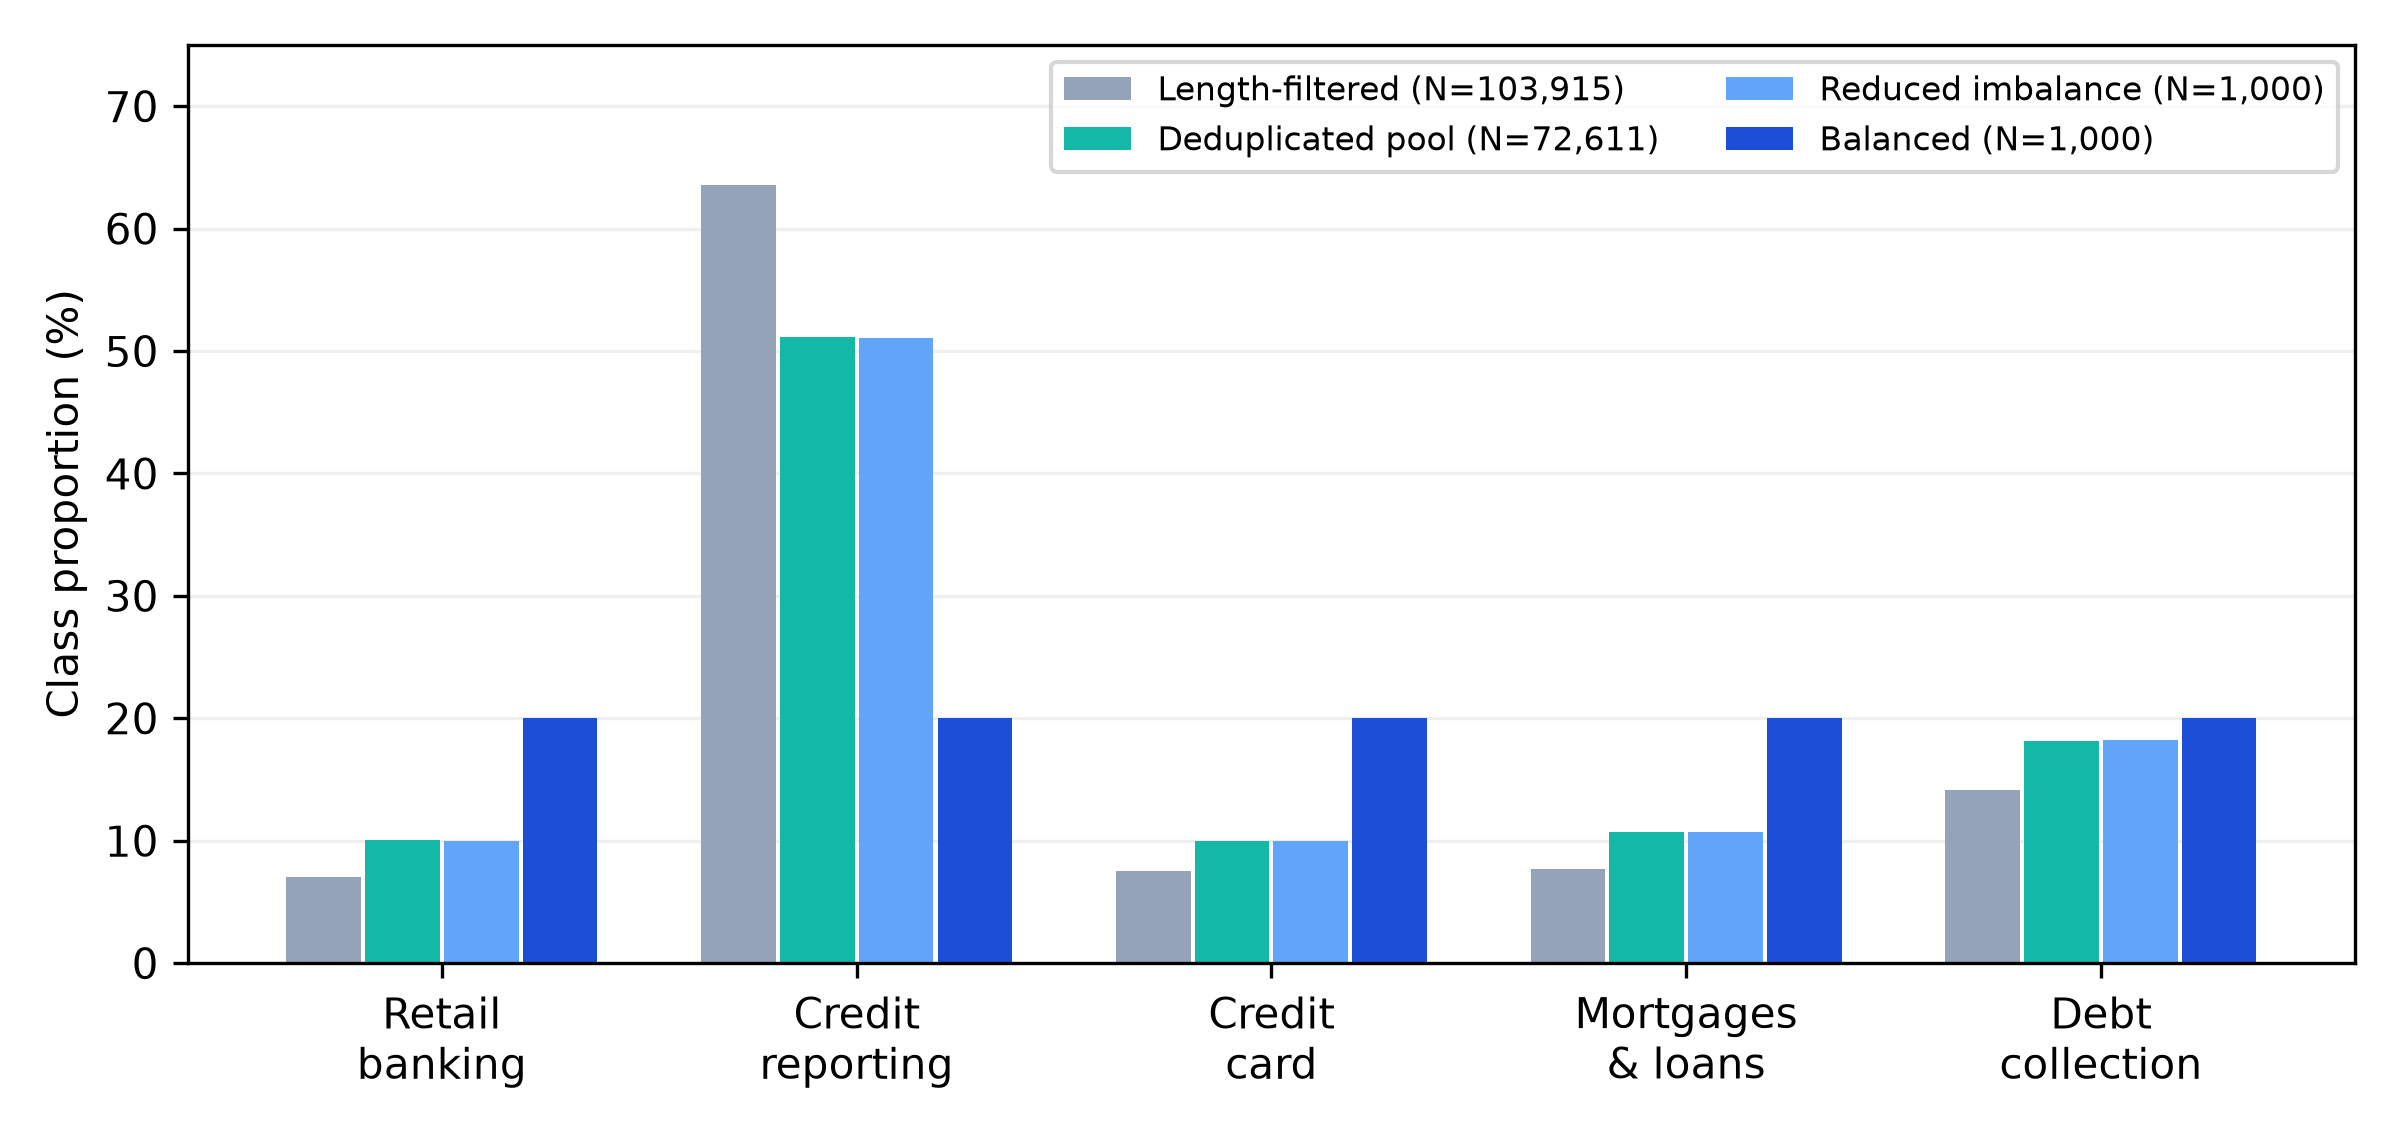
\includegraphics[width=\textwidth]{figures/v2/class_distribution.png}
  \caption{Class proportions (\%) in the length-filtered dataset before
           deduplication ($N{=}103{,}915$), the deduplicated sampling pool
           ($N{=}72{,}611$), the reduced-imbalance experimental subset
           ($N{=}1{,}000$), and the balanced subset ($N{=}1{,}000$).
           Experiment~B rounds the proportions of the deduplicated
           $N{=}72{,}611$ pool, where credit reporting accounts for
           51.15\,\%; the first bars describe the earlier preprocessing stage.}
  \label{fig:class_dist}
\end{figure}

\subsection{Preprocessing Pipeline}

The preprocessing steps, implemented in Python using pandas, are applied
in the following order to every record:

\begin{enumerate}
  \item Drop rows with empty \texttt{product} or \texttt{narrative}.
  \item Retain only records belonging to the five target categories.
  \item Remove narratives longer than 500 characters, reducing processing
        time and GPU memory pressure while avoiding truncation artifacts
        during inference.
  \item Remove exact duplicate narratives before normalisation.
  \item Standardise narrative text: convert to lowercase, remove special
        characters, and normalise whitespace.
\end{enumerate}

\subsection{Experimental Subsets}

Two experimental conditions are defined, each evaluated under a
three-subset, two-length design to describe sampling variation.

\textbf{Experiment~A (Balanced):} Each subset randomly samples 200
records per category ($N=1{,}000$), following the balanced design of
Roumeliotis~et~al.\ \cite{roumeliotis2025think}.

\textbf{Experiment~B (Reduced imbalance):} Each $N=1{,}000$ subset
rounds the deduplicated-pool proportions to 51.1\,\% credit reporting,
18.2\,\% debt collection, 10.7\,\% mortgages/loans and
10.0\,\% each for retail banking and credit cards. A majority-only
classifier would achieve 51.1\,\% accuracy. This condition measures
sensitivity to class proportions within the processed pool, rather
than representing deployment traffic.

\textbf{Test-subset and narrative-length design:}
Each condition is replicated with three subset identifiers (1, 2,
and 3) and at two narrative character-length limits (250 and 500
characters), yielding 12 datasets per model and 132 inference runs in
total (11~models $\times$~3~test~subsets~$\times$~2~conditions~$\times$~2~length
limits). The 250-character subsets contain exactly the same records in
the same order as their 500-character counterparts, with narratives
truncated to 250 characters. Balanced and reduced-imbalance subsets
share 2,067 of their 3,000 records per condition at 500 characters,
yielding 3,933 unique full-text inputs across both conditions. They
are therefore not independent replications.

The eleven-model GGUF benchmark tables use the 500-character variant
and mean~$\pm$~standard deviation across the three test subsets. HF
adaptation comparisons instead pool 3,000 predictions per mode and
condition, with paired cluster-bootstrap intervals. The three test
identifiers are distinct from the three LLM adaptation training seeds.
The 250-character runs provide a narrative-length
sensitivity check discussed in Section~\ref{sec:sensitivity}.
These subsets describe variation within this short-narrative population;
they do not establish stability across training seeds, prompts or future data.

All evaluation protocols use subsets of the same fixed benchmark.
Model selection for adaptation considers zero-shot performance and
deployment characteristics (Section~\ref{sec:qlora_methods});
checkpoint and hyperparameter selection use the separate validation
set (Section~\ref{sec:supervised_methods}). Supplementary
Fig.~\ref{S-fig:char_hist} describes the source narrative-length distribution.


% =============================================================
\section{Experimental Setup}
\label{sec:setup}

The three LLM experimental arms answer distinct questions. The
eleven-model GGUF benchmark evaluates zero-shot deployment configurations; paired HF
runs estimate adaptation gains against matched frozen bases; the GGUF
thinking control estimates policy differences on a fixed 500-input
subset. Absolute scores across these arms are not directly
interchangeable because artifacts, inference settings and evaluation
samples differ. Adaptation and thinking gains are therefore interpreted
within their respective paired controls.

\subsection{Infrastructure}

The supervised classifier and paired HF adaptation experiments run on an
Ubuntu workstation with an Intel Core i7-14700 processor, 32\,GB RAM,
and an NVIDIA GeForce RTX~5060~Ti with 16\,GB VRAM. The adaptation
environment uses Python~3.12, PyTorch~2.14.1, Transformers~5.18.0,
PEFT~0.21.2 and bitsandbytes~0.50.2. Model revisions, dataset and adapter
SHA-256 hashes, package versions and run statuses are saved. The HF
evaluation uses cached weights in offline mode; complaint narratives
are not sent to a third-party model service.

The GGUF zero-shot benchmark uses Ollama \cite{ollama2026docs}, a self-contained serving runtime
that manages model loading, KV-cache management, and the local REST API.
Its Python inference script communicates through a local REST endpoint.
GGUF request timing and HF generation timing use different runtime
settings and measurement boundaries and are reported separately.

\subsection{Models}

Table~\ref{tab:models} lists the eleven Ollama tags and reported
artifact sizes. They were evaluated without task-specific fine-tuning.
The families include LLaMA \cite{grattafiori2024llama3}, Mistral
\cite{jiang2023mistral}, Gemma~2/4 \cite{team2024gemma2,google2026gemma4card}, Phi
\cite{abdin2024phi4}, Qwen \cite{qwen2025qwen3}, DeepSeek
\cite{deepseekllm2024,guo2025deepseekr1} and OpenAI's open-weight
gpt-oss \cite{openai2025gptoss}; the latter uses local weights, without
a proprietary API.

Model tags do not isolate architecture, parameter count or reasoning.
Gemma~4 supports configurable thinking \cite{google2026gemma4card},
but its mode was not recorded in the eleven-model benchmark. Its leading
zero-shot point estimate therefore cannot be attributed to thinking
being enabled or disabled. DeepSeek's current 8B/14B
tags map to R1-0528-Qwen3 and R1-Distill-Qwen2.5, respectively
\cite{ollama2026deepseekregistry}; missing artifact digests prevent
a clean size comparison. Current metadata also shows differing
quantisation formats, including Q4\_K\_M for Qwen3~8B and MXFP4 for
gpt-oss. Registry tags alone do not uniquely identify the evaluated weights. Artifact sizes are not peak runtime VRAM measurements.
The HF adaptation and GGUF thinking controls pin artifacts and
report their protocols separately.

\begin{table}[!t]
  \renewcommand{\arraystretch}{1.2}
  \caption{Open-weight model builds evaluated in the GGUF benchmark. Reported
           artifact sizes are listed; peak runtime VRAM was not recorded. Type records
           the original grouping, not a verified per-request thinking flag.}
  \label{tab:models}
  \centering
  \footnotesize
  \setlength{\tabcolsep}{3pt}
  \begin{tabular}{@{}lllrr@{}}
    \toprule
    \textbf{Model} & \textbf{Family} & \textbf{Type} & \textbf{Params} & \textbf{Size} \\
    \midrule
    \texttt{gemma2:9b}         & Google     & Standard  & 9B   & 5.4\,GB \\
    \texttt{gemma4:12b}        & Google     & Unverified & 12B  & 7.6\,GB \\
    \texttt{mistral:7b}        & Mistral    & Standard  & 7B   & 4.4\,GB \\
    \texttt{mistral-nemo:12b}  & Mistral    & Standard  & 12B  & 7.1\,GB \\
    \texttt{llama3.1:8b}       & Meta       & Standard  & 8B   & 4.9\,GB \\
    \texttt{phi4:14b}          & Microsoft  & Standard  & 14B  & 9.1\,GB \\
    \midrule
    \texttt{deepseek-r1:8b}    & DeepSeek   & Reasoning & 8B   & 5.2\,GB \\
    \texttt{deepseek-r1:14b}   & DeepSeek   & Reasoning & 14B  & 9.0\,GB \\
    \texttt{qwen3:8b}          & Alibaba    & Reasoning & 8B   & 5.2\,GB \\
    \texttt{qwen3:14b}         & Alibaba    & Reasoning & 14B  & 9.3\,GB \\
    \texttt{gpt-oss:20b}       & OpenAI     & Reasoning & 20B  & 13.0\,GB \\
    \botrule
  \end{tabular}
\end{table}

\subsection{Prompt Design}

A common task instruction and five-label taxonomy are used across
the LLM experiments, with arm-specific chat templates, thinking policies
and generation limits rather than identical rendered model inputs.
The instruction follows the JSON-output template
used by Roumeliotis~et~al.\ \cite{roumeliotis2025think} to align
task instructions:

\begin{quote}
\textit{You are an AI assistant specializing in consumer complaint
classification. Your task is to analyze a consumer complaint and
classify it into the most appropriate category from the predefined
list: ["retail\_banking", "credit\_reporting", "credit\_card",
"mortgages\_and\_loans", "debt\_collection"]. Provide your final
classification in the following JSON format without explanations:
\texttt{\{"product": "chosen\_category\_name"\}}. Complaint: [NARRATIVE]}
\end{quote}

For the eleven-model GGUF benchmark, temperature is set to 0 to reduce
sampling variability and improve reproducibility. No explicit
\texttt{top\_p}, \texttt{max\_tokens}, stop-sequence, or model-specific
thinking-mode flags are set; Ollama defaults are used for all other
decoding parameters. Although the prompt asks for JSON without
explanations, some reasoning-oriented builds may still emit
intermediate text before the final answer. The inference script
therefore extracts the final JSON object from the response by searching
for the last valid \texttt{\{"product": "..."\}} occurrence using a
regular expression, accounting for models that prepend reasoning traces
before the answer.

The GGUF benchmark script retries an HTTP failure once and counts unresolved
errors. It saves at most 2,000 response characters, replaces newlines
with spaces and falls back to a category mentioned in prose if JSON
extraction fails. Separate thinking text, termination reasons and
token counts were not retained. Section~\ref{sec:audit} checks whether
strict JSON reparsing changes the classifications.

\subsection{Evaluation Metrics}

Each GGUF benchmark run scores all $N=1{,}000$ predictions using accuracy,
weighted precision, recall and F1. Macro-F1 gives equal weight to the
five classes and complements weighted metrics under imbalance.
Invalid outputs include parsing failures and out-of-taxonomy labels;
they remain errors in the full denominator. Mean request latency
and invalid-output counts accompany the scores. All local runs incur
zero model-API fees; local compute and electricity costs are not estimated.

% =============================================================
\subsection{Supervised Data and Classifier Controls}
\label{sec:supervised_methods}

To assess whether an LLM is warranted when labelled data are available,
we add TF-IDF/LinearSVC and fine-tuned DistilBERT
\cite{sanh2019distilbert} baselines. All twelve saved test sets remain
unchanged. Training and validation use separate balanced sets of
20,000 and 2,000 records, respectively. We exclude normalised exact
matches and shared 250-character prefixes with any test narrative,
discard 133 conflicting-label text groups, and screen near duplicates
using 128-permutation MinHash retrieval followed by exact word-trigram
Jaccard similarity at threshold 0.85. This excludes 496 additional
test-similar records and 28 validation-similar training candidates.
The approximate retrieval cannot guarantee removal of every paraphrase.

The preserved test narratives are reserved before drawing training and
validation records. Test-text matching is an exclusion constraint during
split construction, not a source of fitted features. Verification finds
zero normalised exact or shared 250-character-prefix matches between
training, validation and tests at all four training budgets. Identity checks
use SHA-256 hashes of normalised text and its 250-character prefix;
the saved source index is a local CSV index, not a CFPB complaint identifier.
Split hashes are recorded in a manifest; test-file hashes are rechecked
before paired HF evaluation. Supplementary Section~\ref{S-sec:split_integrity}
details the split counts, sampling seeds and statistical units.

Nested balanced training subsets of 500, 2,000, 10,000, and 20,000
records are used for the classical learning curve. TF-IDF uses word
unigrams/bigrams, sublinear term frequencies, minimum document
frequency 2, and at most 100,000 features. Vocabulary and IDF weights
are fitted exclusively on each training subset; validation and test
inputs are transformed without refitting. This differs from the fixed,
non-learned lowercasing and character/whitespace normalisation.
LinearSVC's $C$ is selected
from $\{0.1,1,10\}$ by validation weighted F1. Warm serial CPU latency includes vectorisation and prediction.

The encoder is \texttt{distilbert/distilbert-base-uncased}, pinned to
the revision listed in the supplementary material. The 20,000-record
and fixed 500-record controls train for three epochs with learning rate
$2\times10^{-5}$, batch size 16, weight decay 0.01, a 256-token cap,
and 10\,\% warmup.
The checkpoint with highest validation weighted F1 is selected.
Training seeds are distinct from the three saved test-subset identifiers.
Within each supervised fit, checkpoint and hyperparameter selection
use the separate validation set, not test performance.
The training and prediction artifacts report exact model commits,
training time, peak allocated VRAM, and warm serial GPU latency.

We additionally train DistilBERT on the identical 500-record subset
with three training seeds and the same 2,000-record validation set.
A fixed three-epoch control had a validation trajectory that was still
improving, motivating a separate
convergence control before inspecting its test scores. This control
allows at most 30 epochs, uses patience 5 on validation weighted F1,
and selects the best validation checkpoint. All other encoder settings
are retained; original three-epoch outputs are preserved separately.
This matches label budgets, not training-update or compute budgets.

All supervised budgets use an additional 2,000 validation labels: total
label counts are 2,500, 4,000, 12,000 and 22,000 for the classical
training budgets. Each LLM adapter fit likewise uses 2,500 labels in
total. A training budget is not the total annotation requirement.
Matching label availability does not equate validation objectives,
fit counts or compute effort (Supplementary Section~\ref{S-sec:split_integrity}).

\subsection{Controlled Lightweight LLM Adaptation}
\label{sec:qlora_methods}

We select Gemma~4~12B, Qwen3~14B and Phi-4~14B to represent the leading
zero-shot GGUF model, a configurable-thinking model and a fast
generative classifier. This exploratory choice uses benchmark outcomes
and deployment characteristics; adaptation findings are conditional on
these selected models, rather than an independent model-selection test.
The HF artifacts are
\texttt{google/gemma-4-12B-it}, \texttt{Qwen/Qwen3-14B} and
\texttt{microsoft/phi-4}. Their exact revisions are listed in the
supplementary material. Adaptation gains use matched HF base
predictions from the same pinned weights and inference settings.

Each model uses the same balanced 500-record training subset (100 per
class) and the common 2,000-record validation set (400 per class),
prepared with the test-exclusion procedure in Section~\ref{sec:supervised_methods}.
Reported training budgets exclude the additional validation labels.
We use LoRA \cite{hu2021lora} with rank 8, scaling factor 16 and dropout
0.05, applied to attention and feed-forward projections. Gemma and
Qwen use separate query/key/value, output, gate/up/down projections;
Phi uses fused QKV and gate/up projections plus output/down projections.
QLoRA \cite{dettmers2023qlora} freezes NF4 double-quantised linear
weights with BF16 compute. Unquantised matrices remain BF16 and
one-dimensional normalisation parameters FP32. Only adapter weights
are updated.

Training uses seeds 1, 2 and 3 on the same training and validation records,
each with three epochs, batch size 1, gradient accumulation
16, learning rate $2\times10^{-4}$, paged 8-bit AdamW, cosine decay,
three warmup steps, gradient checkpointing and a 512-token cap.
Loss is restricted to the assistant's target JSON and end-of-turn token;
the prompt is masked. All training and validation sequences fit without
truncating a target. Each fit completes 96 optimiser steps. Minimum completion-only
validation loss, evaluated after each epoch, selects and records a
checkpoint separately for each fit. Test scores do not guide selection.

Paired inference loads one NF4 PEFT model and enables/disables its
unmerged adapter. Both modes retain identical frozen weights,
normalisation, chat template and precision. The same five-category
prompt is rendered through each pinned model's chat template with
thinking disabled. Greedy decoding uses a 64-new-token cap and the
model's end-of-turn token, with independent KV caches for every call.
Inputs are left-padded with attention masks. Maximum batch size is 32.
Phi's seed-1 evaluation falls back to 16 after a long-input memory
failure; seeds 2 and 3 retain a maximum of 32. Both modes of
a pair use the same actual batch size. Full raw responses, token counts,
output-limit flags, source hashes and original row indices are saved.
A JSON decoder accepts the last explicit string-valued \texttt{product}
field; parse failures and out-of-taxonomy labels remain errors.

The full design yields 216,000 predictions: three models, three training
seeds, two modes and twelve preserved 1,000-record files. Metrics pool the three test subsets
within each condition/length.

We compute unadjusted 95\,\% percentile
intervals from 5,000 paired bootstrap resamples
using identical normalised-text-cluster weights for both modes,
stratified by class when cluster labels are consistent. Exact two-sided
McNemar tests compare accuracy on unique source inputs, retaining the
first subset/index for duplicates; conflicting-label inputs would be
excluded only from this test. Holm correction covers all 36 model--training-seed--condition--length
comparisons; these are paired tests within one design, not 36 independent
experimental replications. Supplementary Section~\ref{S-sec:split_integrity}
defines the text clusters and conflicting-label handling.

Metrics are calculated per fit, then mean and sample
standard deviation are reported over the three fits. No independence between
overlapping conditions or length variants is assumed. Bootstrap confidence intervals describe test-output uncertainty within
a fit; training-seed variability is reported separately. Repeated model
fits are never pooled into 9,000 independent test observations.
The frozen base is re-evaluated in every paired run. Its small variation
for Phi is run/batch variation rather than variation in trained base
weights; between-fit adapter dispersion is conditional on these runs.

Training/validation runtime excludes initial weight loading; peak
allocated CUDA memory includes the loaded model and training operations.
Serving latency is measured separately on the first 20 records per
class in the first balanced 500-character subset (100 per mode/model),
sorted back to their original indices, after a warmup call in each mode.
Batch-1 timing includes prompt rendering, tokenisation and synchronised
CUDA generation, excluding output decoding and network overhead.
Full-test batch wall time divided by batch size is saved as amortised
time and is not interpreted as serial latency.


\section{Results}
\label{sec:results}

We first report direct classifiers at explicit label budgets, followed
by matched HF adaptation and controlled GGUF thinking policies.
The eleven-model zero-shot benchmark then supplies context
on model configurations, class imbalance and published API results.

\subsection{Supervised Baselines on the Preserved Test Sets}
\label{sec:supervised}

The classifier controls use the splits and settings in
Section~\ref{sec:supervised_methods}.
Table~\ref{tab:supervised} summarises the learning curve and the
DistilBERT results at both training-label budgets.
The 20,000-record encoder fits take approximately 80~s each and peak
at 1.30~GiB allocated memory; their warm serial inference averages
2.07~ms on the same workstation used for the HF adaptation benchmark.

\begin{table}[tb]
\centering
\caption{Supervised balanced-test performance. F1 is computed on the
pooled 3,000 records; DistilBERT values average three separate model fits.
Every row uses 2,000 additional validation labels; total labelled budgets
are training records plus 2,000. Latency is warm serial end-to-end feature/token preparation and inference.}
\label{tab:supervised}
\begin{tabular}{lrrr}
\toprule
Model & Training records & Weighted F1 & Latency (ms) \\
\midrule
TF-IDF/SVM (CPU) & 500 & 0.7546 & 0.29 \\
TF-IDF/SVM (CPU) & 2,000 & 0.7908 & 0.29 \\
TF-IDF/SVM (CPU) & 10,000 & 0.8241 & 0.28 \\
TF-IDF/SVM (CPU) & 20,000 & 0.8291 & 0.29 \\
DistilBERT (3 epochs) & 500 & $0.5329\pm0.1522$ & 2.06 \\
DistilBERT (early stop) & 500 & $0.7150\pm0.0208$ & 2.07 \\
DistilBERT (GPU) & 20,000 & $0.8244\pm0.0046$ & 2.07 \\
\botrule
\end{tabular}
\end{table}

Paired two-sided McNemar comparisons against the Gemma~4 GGUF zero-shot
balanced predictions (Table~\ref{tab:results_balanced}) give
Holm-adjusted $p<0.001$ for the 20,000-record
SVM and for each of the three 20,000-record DistilBERT fits,
with positive accuracy differences of 4.67--5.60 percentage points for
these encoder fits. Correction covers all 42
baseline--reference--condition comparisons. This tests accuracy gains,
not F1 differences; the zero-shot and supervised label budgets differ.

Figure~\ref{fig:label_budget} shows the observed training-budget trade-off.
At 500 training records, adapter mean F1 exceeds the label-matched SVM
point estimate. At 2,000 training records, SVM reaches 0.7908, above the
three observed 500-record adapter means, with warm CPU latency below
0.3~ms. This latter comparison uses different total label budgets
(4,000 versus 2,500). The LLM learning curve and a crossover budget
remain unmeasured; these observations do not establish a threshold
beyond which adaptation is unnecessary.

\begin{figure}[tb]
\centering
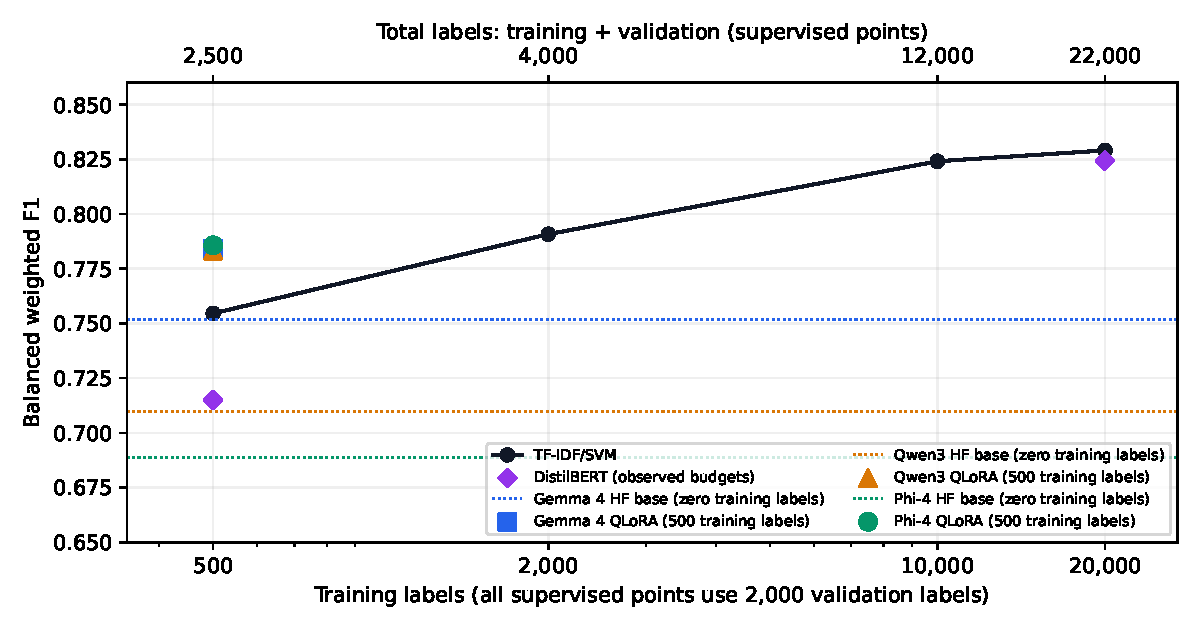
\includegraphics[width=\textwidth]{figures/v2/label_budget_tradeoff.pdf}
\caption{Observed balanced 500-character weighted F1 by training-label
budget (log axis). Direct classifiers additionally use 2,000 validation
labels; the upper axis shows their total annotation requirement. QLoRA
points use 500 training plus 2,000 validation labels. DistilBERT and
QLoRA points are means over three fits; no unmeasured intermediate
encoder or LLM budgets are interpolated. Horizontal HF base references
use zero task-labelled training data and the fixed thinking-off protocol.}
\label{fig:label_budget}
\end{figure}

These supervised comparisons use additional labelled data and
therefore measure a different deployment regime from zero-shot
inference. Their strong performance requires the LLM deployment
recommendations to be conditional on the availability of training
labels. The matched 500-training-label LLM adaptation experiment is
reported in Section~\ref{sec:qlora_results}; higher-budget baselines do not establish equal-budget
superiority. All supervised budgets additionally use the same 2,000
validation labels.

\subsection{QLoRA Adaptation with Three Training Seeds}
\label{sec:qlora_results}
Nine adapter fits completed all twelve preserved tests, giving 216,000
paired base/adapted predictions and 1,800 serial benchmark predictions.
Each fit is evaluated separately on the same 3,000 records per condition;
Table~\ref{tab:qlora_paired} and Fig.~\ref{fig:qlora_paired} report
means and sample standard deviations over three training seeds.
Balanced mean weighted-F1 gains range from 3.21 to 9.72 percentage
points. Adapted means lie between 0.7833 and 0.7857; these nearby point
estimates do not establish model-to-model superiority.
% Generated by export_qlora_manuscript.py from verified saved predictions.
\begin{table}[tb]
\centering
\footnotesize
\setlength{\tabcolsep}{3pt}
\caption{Paired HF base/QLoRA weighted F1 on 500-character tests. Each mode uses 3,000 pooled records; all adapters use 500 training and 2,000 validation records. A: balanced; B: reduced imbalance. Gains and paired 95\,\% intervals are in percentage points.}
\label{tab:qlora_paired}
\begin{tabular}{llrrrr}
\toprule
Model & Condition & Base F1 & QLoRA F1 & $\Delta$ (pp) & 95\,\% CI ($\Delta$) \\
\midrule
Gemma 4 & A & 0.7520 & 0.7803 & +2.83 & [1.75, 3.96] \\
Gemma 4 & B & 0.7730 & 0.7948 & +2.18 & [1.12, 3.22] \\
Qwen3 & A & 0.7099 & 0.7891 & +7.92 & [6.55, 9.34] \\
Qwen3 & B & 0.7278 & 0.7946 & +6.68 & [5.30, 8.07] \\
Phi-4 & A & 0.6883 & 0.7845 & +9.62 & [8.21, 11.07] \\
Phi-4 & B & 0.7456 & 0.7994 & +5.38 & [4.08, 6.68] \\
\bottomrule
\end{tabular}
\end{table}
\begin{table}[tb]
\centering
\footnotesize
\setlength{\tabcolsep}{3pt}
\caption{Local resource measurements for 500-training-record adapters. Latency: warm batch-1 mean on the same 100 balanced 500-character records per mode, including prompt preparation and generation. Training time includes validation/checkpointing and excludes initial weight loading. Memory is peak allocated CUDA memory, not total GPU utilisation.}
\label{tab:qlora_resources}
\begin{tabular}{lrrrr}
\toprule
Model & Base (s) & QLoRA (s) & Train (min) & Peak (GiB) \\
\midrule
Gemma 4 & 0.475 & 0.647 & 34.75 & 7.77 \\
Qwen3 & 0.421 & 0.539 & 41.15 & 10.04 \\
Phi-4 & 0.487 & 0.435 & 40.68 & 9.32 \\
\bottomrule
\end{tabular}
\end{table}


Within this paired test design's 36 model--training-seed--condition--length comparisons,
34 unadjusted 95\,\% paired F1-change intervals exclude zero in the positive direction.
34 accuracy comparisons pass Holm correction across this family
of 36 tests. These within-fit intervals measure uncertainty conditional
on saved test outputs; between-fit variation is reported separately.
The two intervals containing zero are Gemma seed 2 under reduced
imbalance at both character limits; their point gains remain positive,
but a reliable improvement is not established in those two comparisons.
Overlapping conditions and narrative variants are not independent replications.
There are 4 invalid adapted predictions among 108,000 outputs,
compared with 73 invalid base outputs. Invalid responses remain errors.
Supplementary Table~\ref{S-tab:replication_full} reports every fit and condition.

\begin{figure}[tb]\centering
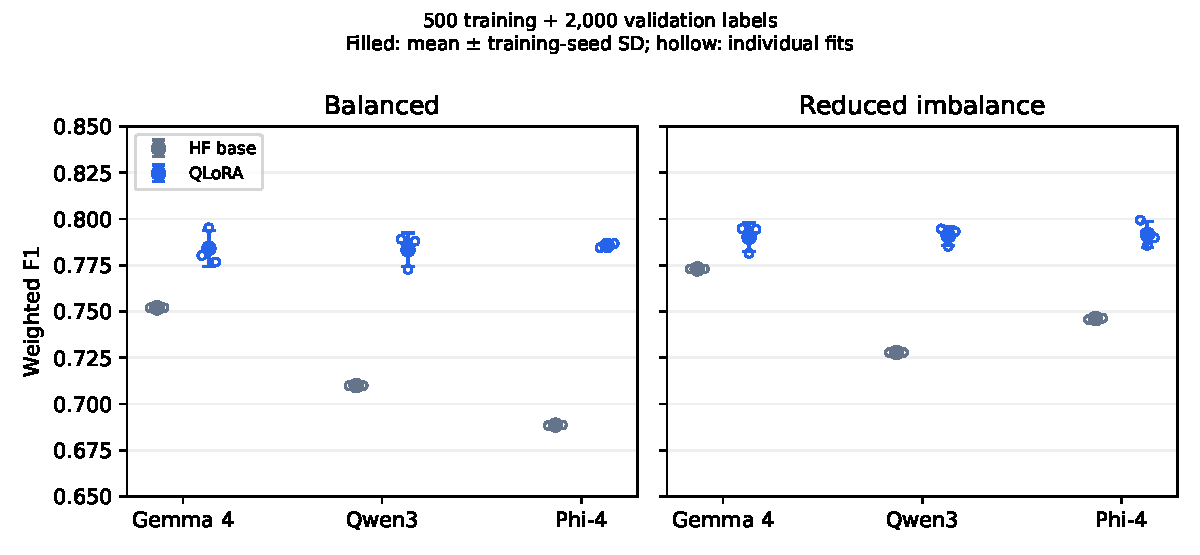
\includegraphics[width=\textwidth]{figures/v2/hf_qlora_multiseed_f1.pdf}
\caption{Matched HF base/adapted mean weighted F1 over three training
seeds on identical 3,000-record tests. Error bars show sample standard
deviation over fits, not bootstrap confidence intervals. Hollow points
show individual fits; the displayed vertical range is 0.65--0.85.}
\label{fig:qlora_paired}\end{figure}

The label-matched classifier comparison uses the same 500 training and
2,000 validation records. The validation-stopped DistilBERT control
has balanced weighted F1 0.7150
$\pm$ 0.0208; the fixed
three-epoch control scores 0.5329
$\pm$ 0.1522.
TF-IDF/SVM scores 0.7546 at the same training-label budget.

Per-fit adapter--classifier F1 differences use paired cluster bootstrap;
accuracy tests correct a separate family of 72 comparisons covering
three models, three fit seeds, two conditions, two lengths and two classifiers.
On balanced 500-character tests, all nine adapter--SVM F1-change
intervals are positive. The corresponding Holm-adjusted accuracy tests
pass for all three Phi fits and two fits each for Gemma and Qwen;
the remaining Gemma/Qwen comparisons have adjusted $p$ values
0.0768 and 0.0812. All nine comparisons with validation-stopped
DistilBERT pass the adjusted accuracy test. These accuracy tests and
unadjusted F1 intervals address different estimands and multiplicity.
The complete differences and adjusted tests are supplied as reproducibility CSVs;
no model-to-model superiority is inferred from point estimates alone.

Supplementary Table~\ref{S-tab:replication_class} reports class F1
over all three fits. Under reduced imbalance, mean adapted credit-card
F1 ranges from 0.6398 to 0.6660 while credit-reporting F1 ranges
from 0.8481 to 0.8511. Thus the high weighted scores do not remove
minority-class weaknesses, including after adaptation.

Table~\ref{tab:qlora_resources} reports training and serial timing.
Adapted balanced serial means range from 0.436 to
0.656~s across model averages. These measurements concern
unmerged adapters and a fixed 100-record warm serial benchmark per fit,
not concurrent throughput. The same benchmark records a decrease in
Phi-4's mean output length from 13.01 tokens without its adapter to
9.34 with it; Gemma and Qwen remain near 9.5 and 9.3 tokens in both
modes. Shorter Phi completions are consistent with its latency reduction,
but output length and adapter execution are not independently manipulated,
so their timing contributions cannot be isolated from these measurements.
Supplementary Section~\ref{S-sec:serial_tokens} reports the per-fit counts.
Full-test F1 uses batched outputs; verification scripts compare source
hashes, labels, saved responses and artifacts and record serial/batch
prediction differences separately.

\subsection{Controlled Thinking-On/Off Comparison}
\label{sec:thinking_control}
We evaluate current pinned Gemma~4~12B and Qwen3~14B GGUF artifacts
on the same 500 unique inputs sampled from the first preserved balanced
test subset (100 per class, at most 500 characters). An excluded
ten-record pilot and a pre-evaluation
amendment fix a common 4,096-token output cap, including reasoning.
Within each model, only the thinking flag changes: prompts, artifact,
temperature zero, context and runtime are fixed. Warm serial requests
alternate mode order. Only final-answer JSON is scored; invalid and
length-terminated outputs remain errors. Table~\ref{tab:thinking_control}
reports this base-model control; it is separate from HF adaptation.
\begin{table}[tb]\centering\small
\caption{Thinking policies on the same 500 balanced inputs. Latency
is warm serial HTTP wall time, including full-response transfer and
excluding initial loading; it is separate from HF generation timing.
F1 is weighted and equals macro-F1 under equal class support.
Latency and generated tokens are means; tokens include reasoning.
Invalid outputs remain in the denominator.}
\label{tab:thinking_control}
\begin{tabular}{llrrrr}\toprule
Model & Thinking & F1 & Invalid & Latency (s) & Tokens \\\midrule
Gemma 4 & Off & 0.7298 & 0 & 0.28 & 13.8 \\
Gemma 4 & On & 0.7447 & 14 & 6.19 & 642.8 \\
Qwen3 & Off & 0.6926 & 0 & 0.25 & 9.2 \\
Qwen3 & On & 0.7449 & 0 & 8.43 & 360.1 \\
\botrule\end{tabular}\end{table}
Thinking increases Qwen3's weighted F1 by 5.23 percentage points
(unadjusted paired 95\,\% interval [+1.91, +8.51]); Gemma's change is
1.49 points ([-1.31, +4.19]), leaving its improvement inconclusive.
Exact accuracy McNemar tests, Holm-adjusted across the two models,
give $p=0.004372$ and $p=0.7798$, respectively. These accuracy tests
are distinct from the unadjusted F1 intervals.

Class-level point estimates in Supplementary
Table~\ref{S-tab:thinking_class} increase for all five Qwen3 categories,
whereas Gemma's F1 decreases for mortgages/loans (0.7527 to 0.7312)
and credit cards (0.7400 to 0.7363), despite its positive overall
change. These patterns are descriptive; no class-specific significance
tests were performed.

Mean latency increases from 0.25 to 8.43~s for Qwen3 and from 0.28
to 6.19~s for Gemma. All 14 invalid Gemma thinking-on outputs
(2.8\,\%) exhaust the shared output budget without a final answer;
the other three configurations have none. The comparison therefore
estimates thinking-policy performance under a finite total-token
budget, conditional on this subset and these artifacts. Prompt and
training-seed robustness are outside this comparison. Supplementary Section~\ref{S-sec:thinking_protocol}
provides the protocol and class scores.


\subsection{Zero-Shot GGUF Benchmark: Balanced Evaluation}
\label{sec:zero_shot_results}

Table~\ref{tab:results_balanced} presents the full results for
Experiment~A, reported as means over three test subsets.
Gemma~4 has the highest mean weighted F1 ($0.774\pm0.016$),
followed by Qwen3~14B ($0.750\pm0.011$) and gpt-oss
($0.749\pm0.018$). These are descriptive ranks: small subset standard
deviations do not establish every pairwise difference. Gemma's
unrecorded thinking mode also prevents attributing its result to
reasoning being enabled or disabled.

Phi-4 combines F1~0.706 with low recorded latency. Mistral-Nemo
has the lowest F1 ($0.540\pm0.025$), despite few invalid outputs;
its deficit therefore concerns classification quality in the saved
configuration rather than primarily output format.

\begin{table}[!t]
  \renewcommand{\arraystretch}{1.2}
  \caption{Experiment A Results — Balanced ($N = 1{,}000$, mean of 3 test subsets; sample std in parentheses)}
  \label{tab:results_balanced}
  \centering
  \scriptsize
  \setlength{\tabcolsep}{2pt}
  \begin{tabular}{@{}llrrrrc@{}}
    \toprule
    \textbf{Model} & \textbf{T} & \textbf{Acc.} & \textbf{F1w} & \textbf{F1m} & \textbf{Lat.(s)} & \textbf{OL} \\
    \midrule
    \texttt{gemma4:12b} & U & 0.773{\scriptsize($\pm$.017)} & 0.774{\scriptsize($\pm$.016)} & 0.774 & 17.12 & 3.7 \\
    \texttt{qwen3:14b} & R & 0.751{\scriptsize($\pm$.011)} & 0.750{\scriptsize($\pm$.011)} & 0.750 & 5.73 & 0.0 \\
    \texttt{gpt-oss:20b} & R & 0.748{\scriptsize($\pm$.020)} & 0.749{\scriptsize($\pm$.018)} & 0.749 & 4.13 & 0.0 \\
    \texttt{deepseek-r1:14b} & R & 0.724{\scriptsize($\pm$.006)} & 0.724{\scriptsize($\pm$.007)} & 0.724 & 9.33 & 1.3 \\
    \texttt{qwen3:8b} & R & 0.717{\scriptsize($\pm$.003)} & 0.717{\scriptsize($\pm$.002)} & 0.717 & 5.19 & 0.0 \\
    \texttt{phi4:14b} & S & 0.705{\scriptsize($\pm$.012)} & 0.706{\scriptsize($\pm$.011)} & 0.706 & 0.54 & 1.0 \\
    \texttt{deepseek-r1:8b} & R & 0.684{\scriptsize($\pm$.013)} & 0.683{\scriptsize($\pm$.012)} & 0.683 & 5.14 & 2.0 \\
    \texttt{gemma2:9b} & S & 0.680{\scriptsize($\pm$.006)} & 0.676{\scriptsize($\pm$.008)} & 0.676 & 0.67 & 0.3 \\
    \texttt{mistral:7b} & S & 0.593{\scriptsize($\pm$.002)} & 0.587{\scriptsize($\pm$.004)} & 0.587 & 0.23 & 58.7 \\
    \texttt{llama3.1:8b} & S & 0.578{\scriptsize($\pm$.005)} & 0.587{\scriptsize($\pm$.003)} & 0.587 & 2.97 & 66.7 \\
    \texttt{mistral-nemo:12b} & S & 0.559{\scriptsize($\pm$.019)} & 0.540{\scriptsize($\pm$.025)} & 0.540 & 0.59 & 0.7 \\
    \botrule
    \multicolumn{7}{l}{\footnotesize T: R=Reasoning, S=Standard, U=Unverified mode. OL=Invalid output mean. Lat.=Mean latency.}
  \end{tabular}
\end{table}

Qwen3~14B, gpt-oss and Qwen3~8B produce no invalid outputs in
these balanced tests. Llama~3.1 and Mistral~7B average 66.7 and 58.7
invalid outputs per subset, respectively. Gemma averages 3.7 empty
responses; retained logs do not identify their cause. Phi-4 averages
one invalid output.

Exploratory exact two-sided McNemar tests compare Gemma with four
leading alternatives in each of three test subsets. Treating these as a
single family of twelve comparisons gives a Bonferroni threshold of
$0.05/12$. Gemma's accuracy advantage over DeepSeek-R1~14B and Qwen3~8B
passes this threshold in all three subsets. Their largest raw p-values
are 0.00296 and 0.000811, respectively. Neither Qwen3~14B nor gpt-oss
passes this twelve-test threshold in any subset. The reference model
was selected after inspecting scores, so these comparisons remain
exploratory and do not establish an F1 ranking or equality between
non-significant pairs.

For Experiment~A, macro-F1 is numerically identical to weighted F1
because all five classes have equal support. Per-class inspection
reveals that even the best model is uneven across labels:
\texttt{gemma4:12b} reaches F1 0.825 on \texttt{retail\_banking} and
0.819 on \texttt{mortgages\_and\_loans} but drops to 0.718 on
\texttt{debt\_collection} and 0.743 on \texttt{credit\_reporting}.
Table~\ref{tab:per_class} reports the leading models' class scores.

Supplementary Fig.~\ref{S-fig:f1_bar} shows the balanced F1 distribution.
Supplementary Figs.~\ref{S-fig:conf_best}, \ref{S-fig:conf_phi4}, and
\ref{S-fig:conf_worst} show confusion matrices for gpt-oss, Phi-4,
and DeepSeek-R1~14B, with invalid outputs in a separate error column.
Debt collection is frequently predicted as credit reporting in these
matrices, even for models with almost no invalid outputs. Llama~3.1's larger invalid-output
count primarily reflects refusals rather than invented category names.

\subsection{Experiment B: Reduced-Imbalance Evaluation}

Table~\ref{tab:results_imbalanced} reports three-subset means for
Experiment~B. All eleven models have numerically higher accuracy and
weighted F1 than in A. Gpt-oss leads with F1~$0.782\pm0.016$,
followed by Gemma ($0.779\pm0.014$) and Qwen3~14B
($0.772\pm0.013$). Llama and Mistral retain substantial invalid-output
counts. Higher aggregate scores under different class proportions
do not establish improved robustness.

\begin{table}[!t]
  \renewcommand{\arraystretch}{1.2}
  \caption{Experiment B Results — Reduced imbalance ($N = 1{,}000$, mean of 3 test subsets; sample std in parentheses)}
  \label{tab:results_imbalanced}
  \centering
  \scriptsize
  \setlength{\tabcolsep}{2pt}
  \begin{tabular}{@{}llrrrrc@{}}
    \toprule
    \textbf{Model} & \textbf{T} & \textbf{Acc.} & \textbf{F1w} & \textbf{F1m} & \textbf{Lat.(s)} & \textbf{OL} \\
    \midrule
    \texttt{gpt-oss:20b} & R & 0.782{\scriptsize($\pm$.017)} & 0.782{\scriptsize($\pm$.016)} & 0.740 & 4.01 & 0.0 \\
    \texttt{gemma4:12b} & U & 0.776{\scriptsize($\pm$.015)} & 0.779{\scriptsize($\pm$.014)} & 0.741 & 10.61 & 2.7 \\
    \texttt{qwen3:14b} & R & 0.772{\scriptsize($\pm$.012)} & 0.772{\scriptsize($\pm$.013)} & 0.730 & 5.53 & 0.0 \\
    \texttt{qwen3:8b} & R & 0.766{\scriptsize($\pm$.008)} & 0.762{\scriptsize($\pm$.007)} & 0.719 & 6.97 & 0.3 \\
    \texttt{phi4:14b} & S & 0.753{\scriptsize($\pm$.003)} & 0.754{\scriptsize($\pm$.002)} & 0.696 & 0.58 & 0.0 \\
    \texttt{deepseek-r1:14b} & R & 0.746{\scriptsize($\pm$.017)} & 0.748{\scriptsize($\pm$.015)} & 0.700 & 7.32 & 0.3 \\
    \texttt{deepseek-r1:8b} & R & 0.738{\scriptsize($\pm$.012)} & 0.731{\scriptsize($\pm$.011)} & 0.677 & 4.46 & 2.3 \\
    \texttt{gemma2:9b} & S & 0.720{\scriptsize($\pm$.012)} & 0.719{\scriptsize($\pm$.014)} & 0.656 & 0.67 & 0.3 \\
    \texttt{mistral-nemo:12b} & S & 0.653{\scriptsize($\pm$.011)} & 0.641{\scriptsize($\pm$.013)} & 0.538 & 0.59 & 0.7 \\
    \texttt{mistral:7b} & S & 0.649{\scriptsize($\pm$.010)} & 0.661{\scriptsize($\pm$.010)} & 0.566 & 0.23 & 42.3 \\
    \texttt{llama3.1:8b} & S & 0.632{\scriptsize($\pm$.006)} & 0.647{\scriptsize($\pm$.012)} & 0.564 & 0.56 & 57.3 \\
    \botrule
    \multicolumn{7}{l}{\footnotesize T: R=Reasoning, S=Standard, U=Unverified mode. OL=Invalid output mean. Lat.=Mean latency.}
  \end{tabular}
\end{table}

Macro-F1 exposes the difference from weighted F1: gpt-oss scores
0.740 versus 0.782, and Llama~3.1 scores 0.564 versus 0.647.
Class-specific scores in Table~\ref{tab:per_class} show where the
majority class masks weaker minority performance.

\subsection{Cross-Experiment Comparison}

Fig.~\ref{fig:comparison_ab} provides a side-by-side view of accuracy
across both experiments. All models improve numerically from
Experiment~A to Experiment~B. \texttt{mistral-nemo:12b} has the largest
gain ($\Delta$acc~$=+0.094$), despite few invalid outputs.
\texttt{mistral:7b} ($+0.055$) and \texttt{llama3.1:8b} ($+0.054$)
also improve, but these shifts cannot be attributed solely to invalid
outputs. Equal-prior reweighting separates the arithmetic effect of
class proportions from class-conditional performance differences.
The conditions use partly overlapping but non-identical records, so
this does not isolate a causal effect of class imbalance.

\begin{figure}[tb]
  \centering
  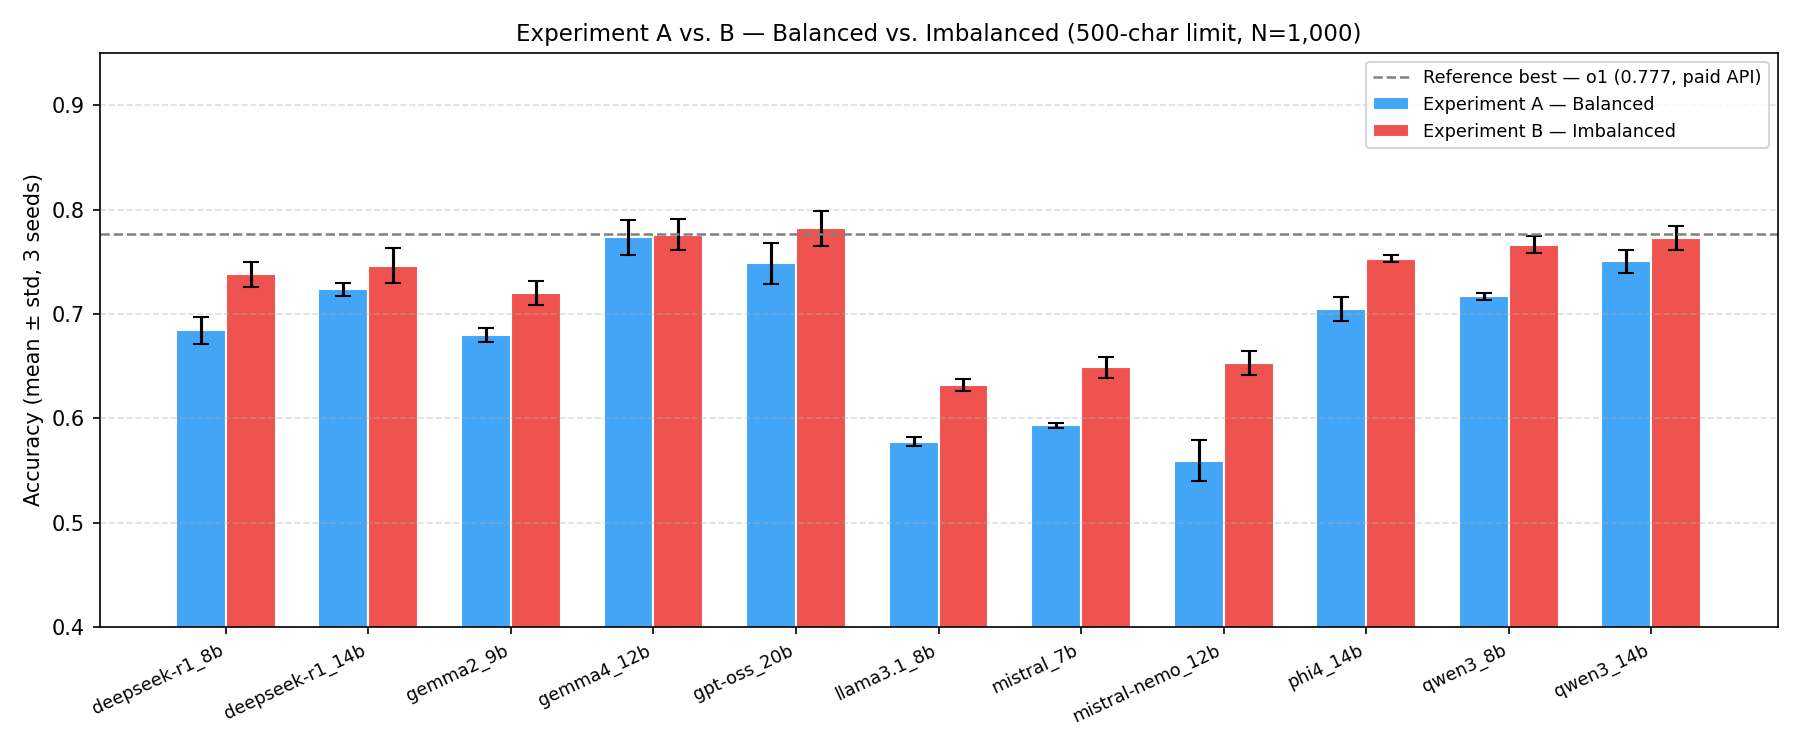
\includegraphics[width=\textwidth]{figures/v2/comparison_A_vs_B.png}
  \caption{Accuracy comparison (mean~$\pm$~sample std over 3 test subsets)
           across Experiment~A (Balanced, blue) and Experiment~B (Imbalanced, red)
           for all models ($N{=}1{,}000$). The dashed reference line marks
           the best published paid-API result (o1, 0.777)
           from \cite{roumeliotis2025think}. The upward shift
           in Experiment~B partially reflects class imbalance and does not isolate improved class-conditional performance.}
  \label{fig:comparison_ab}
\end{figure}

\subsection{Comparison with Paid-API Models}

Table~\ref{tab:vs_reference} places local balanced results alongside
the published API results of Roumeliotis~et~al.\
\cite{roumeliotis2025think}; Supplementary Fig.~\ref{S-fig:vs_reference}
shows the complete comparison. Gemma's mean F1~0.774 is numerically
close to GPT-4.5 (0.7763) and o1 (0.7764). Qwen3~14B and gpt-oss
have point estimates above GPT-4o (0.7358) and below Claude~3.7
Sonnet (0.7626). Exact reference test identifiers and predictions
are unavailable, so these cross-study observations establish neither
paired superiority nor statistical equivalence.

The table compares the model-API fees reported by the reference study: o1 was reported at
\$24.24 per thousand predictions, while local inference incurs no
third-party model-API charge. Hardware, electricity and maintenance
are excluded from this comparison.

\begin{table}[!t]
  \renewcommand{\arraystretch}{1.2}
  \caption{Balanced zero-shot performance and third-party API fees per
  1,000 predictions. Commercial scores and reported fees are from
  \cite{roumeliotis2025think}; local scores summarise three 1,000-record
  subsets. Hardware, electricity and maintenance are excluded.}
  \label{tab:vs_reference}
  \centering
  \scriptsize
  \setlength{\tabcolsep}{2pt}
  \begin{tabular}{@{}llrrl@{}}
    \toprule
    \textbf{Model} & \textbf{Source} & \textbf{Accuracy} & \textbf{F1} & \textbf{API fee/1k} \\
    \midrule
    o1                          & Paid API & 0.777             & 0.7764            & \$24.24 \\
    GPT-4.5                     & Paid API & 0.774             & 0.7763            & \$12.32 \\
    \textbf{\texttt{gemma4:12b}}& \textbf{Open-weight} & $\mathbf{0.773{\pm}.017}$ & $\mathbf{0.774{\pm}.016}$ & \textbf{\$0.00} \\
    Claude~3.7~Sonnet           & Paid API & 0.765             & 0.7626            & \$0.64 \\
    Gemini~2.0~Flash            & Paid API & 0.758             & 0.7586            & \$0.04 \\
    \texttt{qwen3:14b}          & Open-weight & $0.751{\pm}.011$ & $0.750{\pm}.011$ & \$0.00 \\
\texttt{gpt-oss:20b}        & Open-weight & $0.748{\pm}.020$ & $0.749{\pm}.018$ & \$0.00 \\
    GPT-4o                      & Paid API & 0.736             & 0.7358            & \$0.45 \\
    \texttt{deepseek-r1:14b}    & Open-weight & $0.724{\pm}.006$ & $0.724{\pm}.007$ & \$0.00 \\
    \texttt{qwen3:8b}           & Open-weight & $0.717{\pm}.003$ & $0.717{\pm}.002$ & \$0.00 \\
    \texttt{phi4:14b}           & Open-weight & $0.705{\pm}.012$ & $0.706{\pm}.011$ & \$0.00 \\
    \botrule
  \end{tabular}
\end{table}



\subsection{Narrative Length Sensitivity}
\label{sec:sensitivity}

Supplementary Fig.~\ref{S-fig:size_sensitivity} compares mean accuracy on
250-character-limit versus 500-character-limit narratives for the
balanced condition (both at $N{=}1{,}000$). The overall ranking
is highly stable: no model changes its relative rank by more than
one position between the two length limits. Most models improve by
0--3 percentage points moving from shorter to longer narratives, with
\texttt{deepseek-r1:14b} (+1.6~pp) and \texttt{llama3.1:8b} (+2.8~pp)
showing gains when additional text from the same complaints is retained.

Pairing all 3,000 balanced predictions and applying Holm correction
over 22 model--condition tests gives significant accuracy changes for
\texttt{llama3.1:8b} ($p_{\mathrm{adj}}<0.001$) and
\texttt{qwen3:14b} ($p_{\mathrm{adj}}=0.0234$).
The DeepSeek-R1~14B change does not pass this corrected threshold
($p_{\mathrm{adj}}=0.0879$).
\texttt{gpt-oss:20b} and \texttt{mistral-nemo:12b} show virtually no
change (approximately 0.13~pp and 0~pp, respectively), indicating little observed sensitivity
to narrative length in this range. The stability of the top-cluster
ranking suggests that the ordering is not driven solely by these two
length settings; this does not establish robustness to longer narratives.



\subsection{GGUF Request Latency}

Tables~\ref{tab:results_balanced} and~\ref{tab:results_imbalanced}
report per-request means for the 500-character GGUF tests. In A,
Mistral~7B is fastest (0.23~s),
while Phi-4 has the highest F1 among configurations averaging below
one second (0.54~s, F1~0.706). Gemma is slowest at 17.1~s;
missing thinking and token logs prevent explaining that latency.
These benchmark request means are reported separately from the
paired HF and thinking-control timings. Supplementary Fig.~\ref{S-fig:f1_imbalanced}
provides the complete Experiment~B F1 plot.

\subsection{Per-Class Breakdown for Leading Models}
\label{sec:per_class_metrics}

Table~\ref{tab:per_class} reports per-class F1 for the three leading
models in each experiment, confirming that aggregate weighted F1 masks
important minority-class variation. In Experiment~B, the four
non-credit-reporting categories have lower support (10.0--18.2\,\%)
than credit reporting (51.1\,\%); ``minority'' refers to this support.
All three models
jump to ${\geq}0.84$ F1 on \texttt{credit\_reporting} while minority
classes remain in the 0.65--0.77 range, showing the class-specific variation discussed in Section~\ref{sec:discussion}.

\begin{table}[tb]
  \renewcommand{\arraystretch}{1.2}
  \caption{Per-Class F1 for Leading Models (Exp.~A and~B, mean over 3 subsets of $N{=}1{,}000$)}
  \label{tab:per_class}
  \centering
  \scriptsize
  \setlength{\tabcolsep}{3pt}
  \begin{tabular}{@{}llccccc@{}}
    \toprule
    \textbf{E} & \textbf{Model} &
    \textbf{Retail} &
    \textbf{CreditRep.} &
    \textbf{Card} &
    \textbf{Mortg.} &
    \textbf{Debt} \\
    \midrule
    A & \texttt{gemma4:12b} & 0.8247 & 0.7432 & 0.7634 & 0.8194 & 0.7178 \\
    A & \texttt{qwen3:14b} & 0.7855 & 0.7212 & 0.7296 & 0.8097 & 0.7019 \\
    A & \texttt{gpt-oss:20b} & 0.7939 & 0.7137 & 0.7394 & 0.7953 & 0.7045 \\
    \midrule
    B & \texttt{gpt-oss:20b} & 0.7509 & 0.8527 & 0.6654 & 0.7403 & 0.6919 \\
    B & \texttt{gemma4:12b} & 0.7687 & 0.8452 & 0.6713 & 0.7448 & 0.6769 \\
    B & \texttt{qwen3:14b} & 0.7353 & 0.8438 & 0.6542 & 0.7426 & 0.6719 \\
    \botrule
    \multicolumn{7}{l}{\footnotesize E = Experiment; Mortg. = Mortgages \& Loans.}
  \end{tabular}
\end{table}

% =============================================================
\subsection{Additional Statistical and Output Audit}
\label{sec:audit}

We estimate 95\,\% percentile confidence intervals using 5,000
bootstrap resamples of the pooled 3,000 predictions in each
500-character condition. Resampling is stratified by true class and
clusters identical normalised narratives, so repeated texts receive
the same bootstrap weight. These intervals condition on the saved
test sets and model outputs, and do not include uncertainty about
pre-training, prompt choice, or commercial reference results. The
pooled estimators differ slightly from means of subset-specific F1.
Table~\ref{tab:bootstrap} reports selected balanced-test estimates.

\begin{table}[tb]
\centering
\caption{Pooled balanced weighted F1 with 95\,\% cluster-bootstrap
         confidence intervals ($N=3{,}000$).}
\label{tab:bootstrap}
\begin{tabular}{lrr}
\toprule
Model & Pooled F1 & 95\,\% interval \\
\midrule
\texttt{gemma4:12b} & 0.7738 & [0.7586, 0.7882] \\
\texttt{qwen3:14b} & 0.7498 & [0.7344, 0.7650] \\
\texttt{gpt-oss:20b} & 0.7497 & [0.7344, 0.7652] \\
\texttt{phi4:14b} & 0.7057 & [0.6892, 0.7216] \\
\botrule
\end{tabular}
\end{table}

The published GPT-4o point estimate (0.7358) falls within the local
Qwen3~14B and gpt-oss intervals. This observation does not constitute
a paired comparison or equivalence test, because reference predictions
and sampling uncertainty are unavailable.

To examine class-prior effects, we rescale each row of the pooled
Experiment~B confusion matrix to equal support, retaining invalid
predictions as an additional error column, then recompute metrics.
For \texttt{mistral-nemo:12b}, observed accuracy 0.6530 becomes 0.5562,
close to Experiment~A's 0.5593. For \texttt{gpt-oss:20b}, accuracy
0.7820 becomes 0.7480, close to Experiment~A's 0.7483.
The weighted F1 values similarly change from 0.6413 to 0.5326 and
from 0.7825 to 0.7495, respectively. Thus most of these aggregate
gains can be explained arithmetically by different class proportions;
this is not a causal experiment with the class prior independently manipulated.

Reparsing all 132 saved response files with a JSON decoder, accepting
only an explicit string-valued \texttt{product} field, changes no
in-taxonomy prediction under the retained legacy outputs.
Across all Gemma~4 files, 37 saved responses are empty; their causes
cannot be distinguished without separate thinking and termination logs.
Representative Llama parse errors are explicit refusals, whereas
Mistral~7B often returns parseable labels such as
\texttt{online\_banking} or \texttt{not\_applicable} outside the taxonomy.
These are distinct deployment failures even though both count as errors.


\section{Discussion}
\label{sec:discussion}

\subsection{Thinking, Reliability and Serving Cost}

The controlled experiment in Section~\ref{sec:thinking_control} shows
that thinking has model-dependent value under the same total output
budget. Qwen3 gains 5.23 weighted-F1 percentage points, with a paired
interval excluding zero; Gemma's 1.49-point change is inconclusive.
Mean latency rises approximately 34-fold and 22-fold, respectively.
Gemma also exhausts the output budget on 2.8\,\% of thinking-on
requests. Enabling thinking therefore requires evaluating both final
answer quality and completion reliability. This paired control isolates the thinking-policy comparison within
each fixed model configuration.

Invalid outputs require diagnosis beyond a single failure count.
GGUF benchmark Llama failures often contain refusals, whereas Mistral~7B
often emits valid JSON with unsupported labels. Format constraints
alone would not enforce a correct classification or remove refusals;
their effect was not tested here. Within-family score differences
also mix size, generation, training recipe or backbone, as detailed
in the supplementary material.

\subsection{Label Budgets and Deployment Choices}

At the matched 2,500-label budget (500 training and 2,000 validation),
adapted LLM mean weighted F1 exceeds the SVM point estimate by
approximately 2.9--3.1 percentage points on the balanced tests.
This gain accompanies warm serial latency of 436--656~ms for the
GPU-served LLMs, compared with 0.29~ms for CPU SVM on the same
workstation. The observed trade-off makes response-time requirements
central to model selection. These point estimates do not establish
model-to-model superiority.

With 2,000 training labels plus the same validation budget,
SVM reaches 0.7908; the 20,000-record classifiers
score still higher. These observed regimes support direct classifiers
when suitable labels are available. The unmeasured LLM learning
curve prevents identifying an equal-budget crossover.

Among the GGUF zero-shot configurations, Gemma offers the highest
balanced point estimate, Phi-4 the highest F1 among configurations
averaging below one second, and Qwen3~8B a smaller artifact with few
invalid outputs. These are conditional trade-offs, not deployment
guarantees: latency depends on hardware and runtime settings,
artifact size does not establish runtime memory, and serial means do
not establish tail latency or concurrent throughput.

Local inference avoids third-party model-API fees and keeps new
complaint text on local infrastructure. The cross-study commercial
comparison supplies context rather than proof of equal quality or
total cost savings. Macro-F1 and class scores remain necessary under
imbalance: equal-prior reweighting explains much of Experiment~B's
aggregate gain, and adaptation retains minority-class weaknesses.

\subsection{Limitations}

\textbf{Data and generalisation.} The 500-character filter and
normalisation change the evaluated population and may remove useful
cues. The paired 250/500-character tests address truncation within
short complaints, not performance on naturally longer narratives.
Partly overlapping test conditions are not independent replications.
English narratives, the five-category taxonomy and single instruction
template further limit generalisation;
pre-training contamination cannot be ruled out.

\textbf{Model and training scope.} The eleven-model benchmark lacks
complete artifact digests and thinking logs; differing quantisation,
architectures and training recipes confound broad family comparisons.
The thinking
control pins current artifacts but uses one fixed 500-record subset
and a finite output budget. LLM adaptation uses only 500 training
records and three seeds on fixed training/validation records; LoRA rank
and target-module choices are not ablated. Within-fit test intervals and between-fit
standard deviations do not establish robustness across new training
corpora, prompts or larger label budgets. Every supervised budget
also requires 2,000 validation labels.

\textbf{Operational scope.} HF serial timing uses 100 fixed balanced
examples after warmup and excludes output decoding and network
serving; thinking-control timing includes the full HTTP response.
They are not interchangeable timing boundaries. Full-test HF scores
use batched outputs, which differ from serial predictions in 11 of
1,800 benchmark cases. Concurrent serving and total ownership cost
were not measured. Zero model-API expenditure does not imply free
local computation. Abstention, human escalation and asymmetric
misrouting costs are outside the evaluated routing task.

% =============================================================
\section{Conclusion}
\label{sec:conclusion}

We compared local zero-shot configurations, three-seed QLoRA
adaptation, direct classifiers and controlled thinking policies on
preserved CFPB tests. At 500 training plus 2,000 validation labels,
adapted balanced weighted F1 averages 0.7833--0.7857, improving matched
bases by 3.21--9.72 percentage points. These means exceed the
label-matched SVM point estimate, with higher serial serving latency.
Direct classifiers improve at larger observed budgets; LLM adaptation
beyond 500 records was not evaluated, so the equal-budget crossover
remains unknown.

Thinking improves Qwen3 under the controlled budget, but Gemma's
change is inconclusive and both incur substantial latency increases.
The practical choice depends on label availability, completion
reliability and serving requirements. Minority-class performance
requires separate inspection even after adaptation. Findings remain
conditional on this short-narrative corpus, fixed prompts and measured
serial settings; longer narratives, temporal shift, concurrent throughput,
tail latency and total ownership cost remain unevaluated.

\section*{Declarations}

% ---- Funding Statement ---------------------------------------
\bmhead{Funding}
This research received no external funding.

% ---- Conflict of Interest ------------------------------------
\bmhead{Conflict of interest}
The authors declare that they have no conflict of interest.

% ---- Ethics Approval -----------------------------------------
\bmhead{Ethics approval and consent to participate}
Not applicable: analysis of an existing public corpus involves no participant
recruitment or intervention. Public narratives may retain identifying or
financial information; local processing alone does not ensure privacy.

% ---- Consent for Publication ---------------------------------
\bmhead{Consent for publication}
Not applicable.

% ---- Data Availability ---------------------------------------
\bmhead{Data availability}
The study uses the publicly available CFPB Consumer Complaints dataset
published on Kaggle \cite{tiwari2021cfpb}.

% ---- Materials Availability ----------------------------------
\bmhead{Materials availability}
Not applicable.

% ---- Code Availability ---------------------------------------
\bmhead{Code availability}
The original benchmark repository is available at:
\url{https://github.com/muhammettan28/ConsumerComplaintwithLLMs}
The adaptation pipeline records pinned model revisions, split manifests,
source/adapter hashes and generated run artifacts for reproducibility.

% ---- Author Contributions ------------------------------------
\bmhead{Author contributions}
Muhammet Tan and Halit Bak{\i}r contributed to the study conception,
experimental design, implementation, analysis, and manuscript preparation.

% ---- References ---------------------------------------------
\bibliography{references}

\end{document}
